\section{First tests}
\label{sec:firstTests}
\timeclock{0}{15}

\vspace{10pt}
This section describes how to operate the functionalities of the Yocto-Pictor 
including relays functions, GPS, temperature, humidity, or light sensors values
reading. The second part explains how to use the Yocto-Pictor to
power the computer instead of a \emph{classical} power supply unit.
Finally, instrument pointing and Hypstar measurements thanks to the GUI 
will be described.

\subsection{Prior Set-up of the System and First tests}


If necessary, get the \textit{hotspot connection} working back 
(\ref{sec:wifirugged}) and start the GUI: 

\begin{lstlisting}
python -m hypernets.gui
\end{lstlisting}
Follow those steps to take a spectrum:

\begin{itemize}
	\item Click on \textit{Connection} and activate the relay \#2 
		(figure \ref{fig:gui})
	\item Wait for 20 seconds (instrument boot time) and click on
		\textit{acquisition}
	\item Click on \textit{Show plot} to see the taken spectrum
		(figure \ref{fig:spectrumPlot})
\end{itemize}

\textbf{Note:} in order to display the real axis unit (in nanometre) 
and to calibrate the spectrum. First \textit{dump} the \textit{linearity and
calibration coefficients}, from the radiometer. Let the relay \#2 opened, exit
the GUI and type once command: 

\begin{lstlisting}
python -m hypernets.dump_current_config
\end{lstlisting}

\subsection{Validation Module Testing}

\begin{itemize}
	\item Open the GUI and activate relay \#2, and \#3 (Figure
		\ref{fig:gui}).
	\item Wait for 20 seconds (instrument boot time)
	\item On the pan-tilt section: set-up the tilt to 198°, click on \textit{move}
	\item Press on \textit{Turn VM on}, and \textit{Measure VM}
	\item Visually check if the Validation Module is lighting
	\item The spectrum graph of the measure should appears (Figure
		\ref{fig:spectrumPlot})
\end{itemize}


\begin{figure}[!ht]
  \centering
  \begin{minipage}[b]{0.48\textwidth}
	  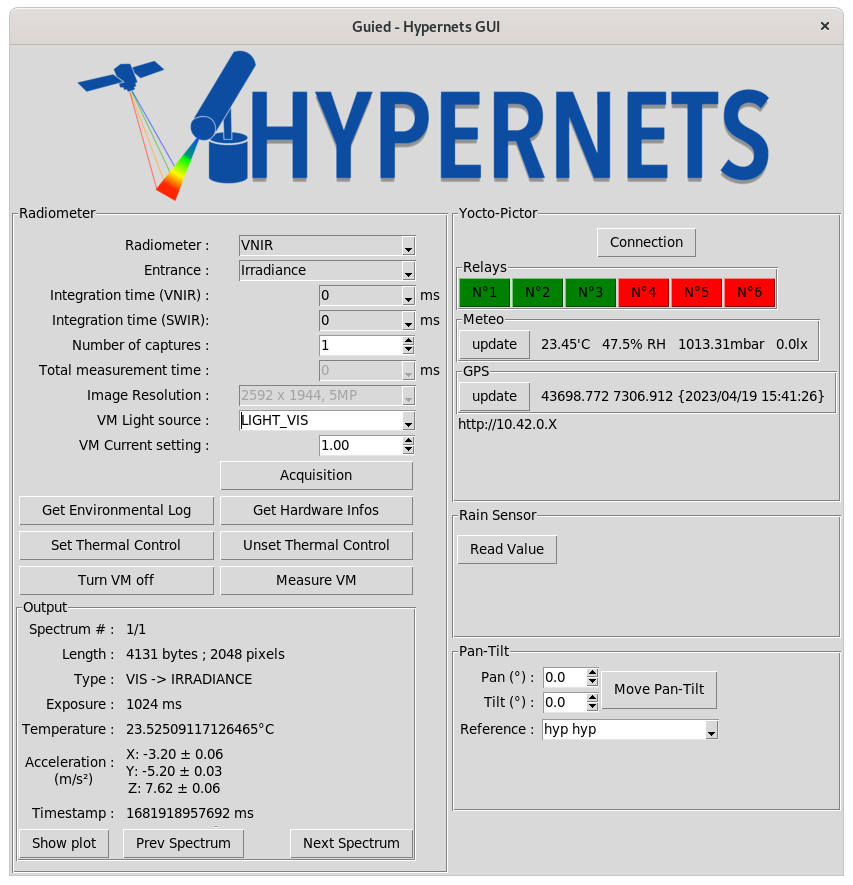
\includegraphics[width=\linewidth]{images/gui_main.png}
	  \vspace{11pt}
	\vspace{-15pt}
	  \caption{Graphical User Interface}
	\label{fig:gui}
  \end{minipage}
  \hfill
  \begin{minipage}[b]{0.48\textwidth}
	  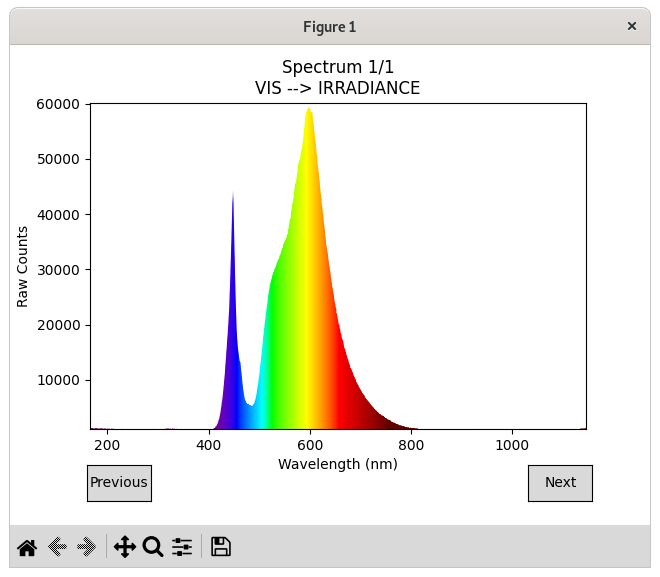
\includegraphics[width=\linewidth]{images/gui_spectrum.png}
	\vspace{-15pt}
	\caption{A Spectrum Plot}
	\label{fig:spectrumPlot}
  \end{minipage}
	\vspace{15pt}
	\vspace{15pt}
	\vspace{15pt}
  \begin{minipage}[b]{\textwidth}
	  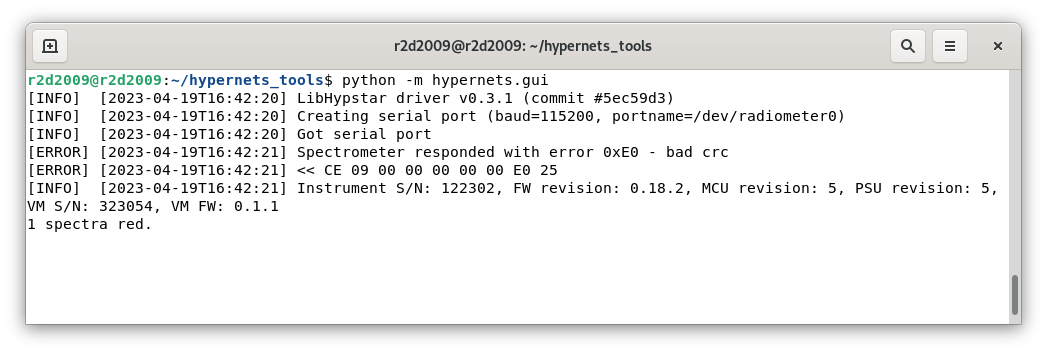
\includegraphics[width=\linewidth]{images/gui_console.png}
	\vspace{-15pt}
	\caption{Some Outputs on the console}
	\label{fig:spectrumPlot}
  \end{minipage}
\end{figure}

\clearpage
\newpage
